\subsubsection{Sourcing Current}
For this second iteration, the low power of the shelf linear regulator has been replaced with a custom discrete 12 A adjustable linear regulator based on the LT3080-1 from Linear Technologies.

The original idea was to make a fully discrete solution, but the relatively low permitted forward voltage drop of the regulator combined with the big output current of 12 A and relatively big range (of at least 2.48 V\textless Vout\textless 5.04 V) made it really challenging to get it stable under all operating conditions. For this several hours of LTspice simulations have been performed to move to a design using an off-the-shelf IC as driver for a high-power transistor shown in Fig. \ref{fig:LT3080-1_LinRegSchematic}.

\begin{figure}[h!]
    \centering
    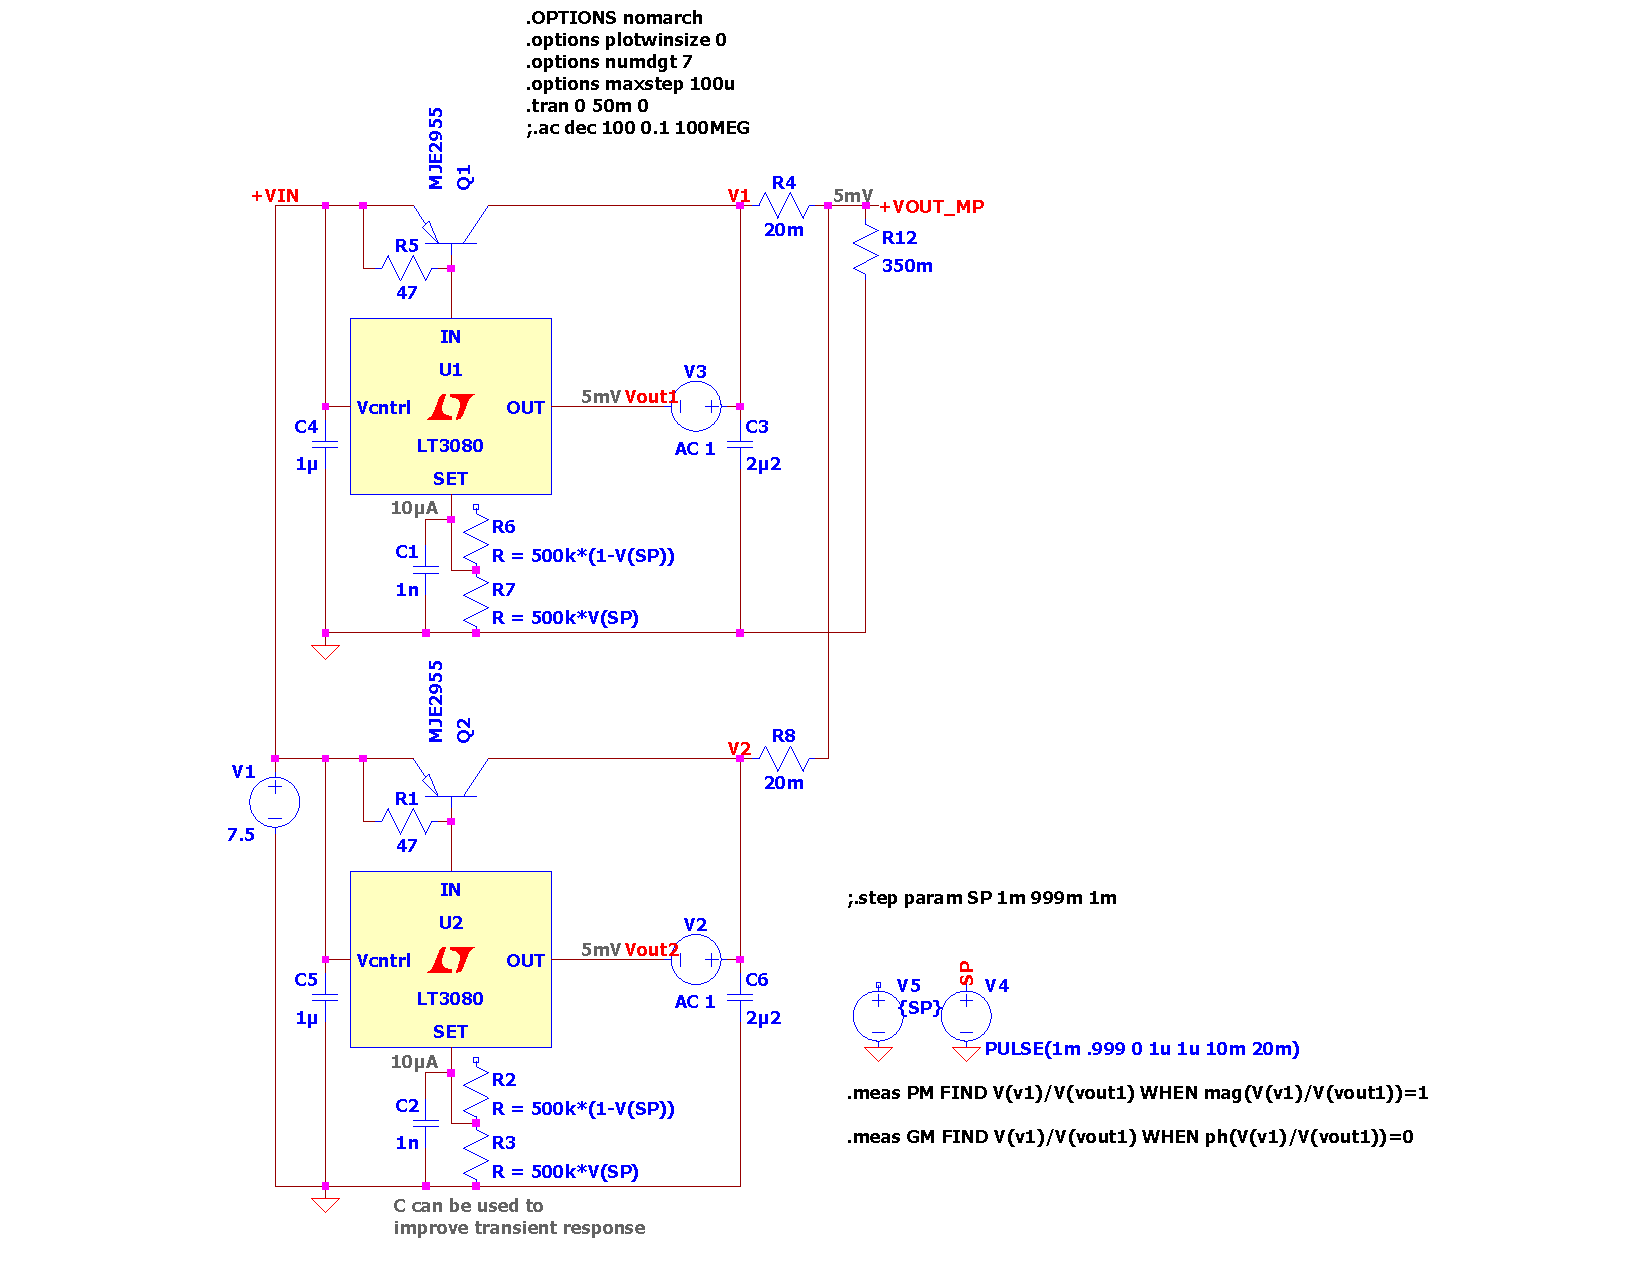
\includegraphics[width=0.45\textwidth]{LT3080-1_LinRegSchematic.pdf}
    \caption{12 A linear regulator design based on the LT3080-1.}
    \label{fig:LT3080-1_LinRegSchematic}
\end{figure}

The working of the circuit is as follows: the LT3080-1 is used as driver for the series pass PNP transistor which is used to amplify the current.
The output voltage can be set by changing the resistance between the set pin of the LT3080-1 and GND since the LT3080-1 incorporates a current source of 10 $\mu$A of which the high side is tied to the non-inverting input of an OpAmp. The output of this OpAmp is connected to its output pin via a NPN transistor and the emitter of this transistor is fed back to the inverting input of the OpAmp for feedback. Thus, the voltage on the output is forced to be the same as the voltage on its set pin, so according to Ohms law by changing the resistance between the set pin and GND, the voltage across the resistor increases and so will the output voltage.

A 1 nF capacitor is placed at each set pin to GND to improve the transient response of the circuit by acting as an energy reservoir. Increasing its value further decreases the transient response since the potentiometer in combination with this capacitor also forms a RC LPF. The series pass PNP transistor is biased with a 47 $\tcohm$ resistor to improve its bandwidth. The 1 $\mu$F input and 2.2 $\mu$F output capacitors are there for stability.

Two of these identical circuits are placed in parallel with their set pins tied together, so they are at the same potential. To accommodate proper current sharing, two 20 m$\tcohm$ series resistors have been added to give some feedback.
The transient response of the linear regulator is shown in Fig. \ref{fig:LT3080-1_Transient-response} and shows that with an input voltage of 7.5 V an output voltage of 0 V up to around 6.9 V can be achieved. The phase margin over set-point (current) is shown in Fig. \ref{fig:LT3080-1_Phase-margin_VS_setpoint} and shows that the regulator is stable. The power dissipation in the main components is shown in Fig. \ref{fig:LT3080-1_PowerDissipation} and provided a good bases for the cooling requirements.

\subsubsection{Sinking Current}
The current sink is based on an OpAmp driving a N-MOSFET in its linear region controlling the current flowing through a sense resistor. The OpAmp changes its output so that the voltage across this sense resistor is equal to its set-point derived from the digital potentiometer. The circuit is shown in \ref{fig:CurrentSinkSchematic} and the working of it is shown in Fig. \ref{fig:CurrentSinkTransient}. The resistor directly at the output of the OpAmp is there to limit the phase shift caused by the gate source capacitance of the MOSFET in combination with its parallel RC snubber. Together these components make the current sink stable in its intended operating region as shown in Fig. \ref{fig:CurrentSinkPM&GM}.

\begin{figure}[h!]
    \centering
    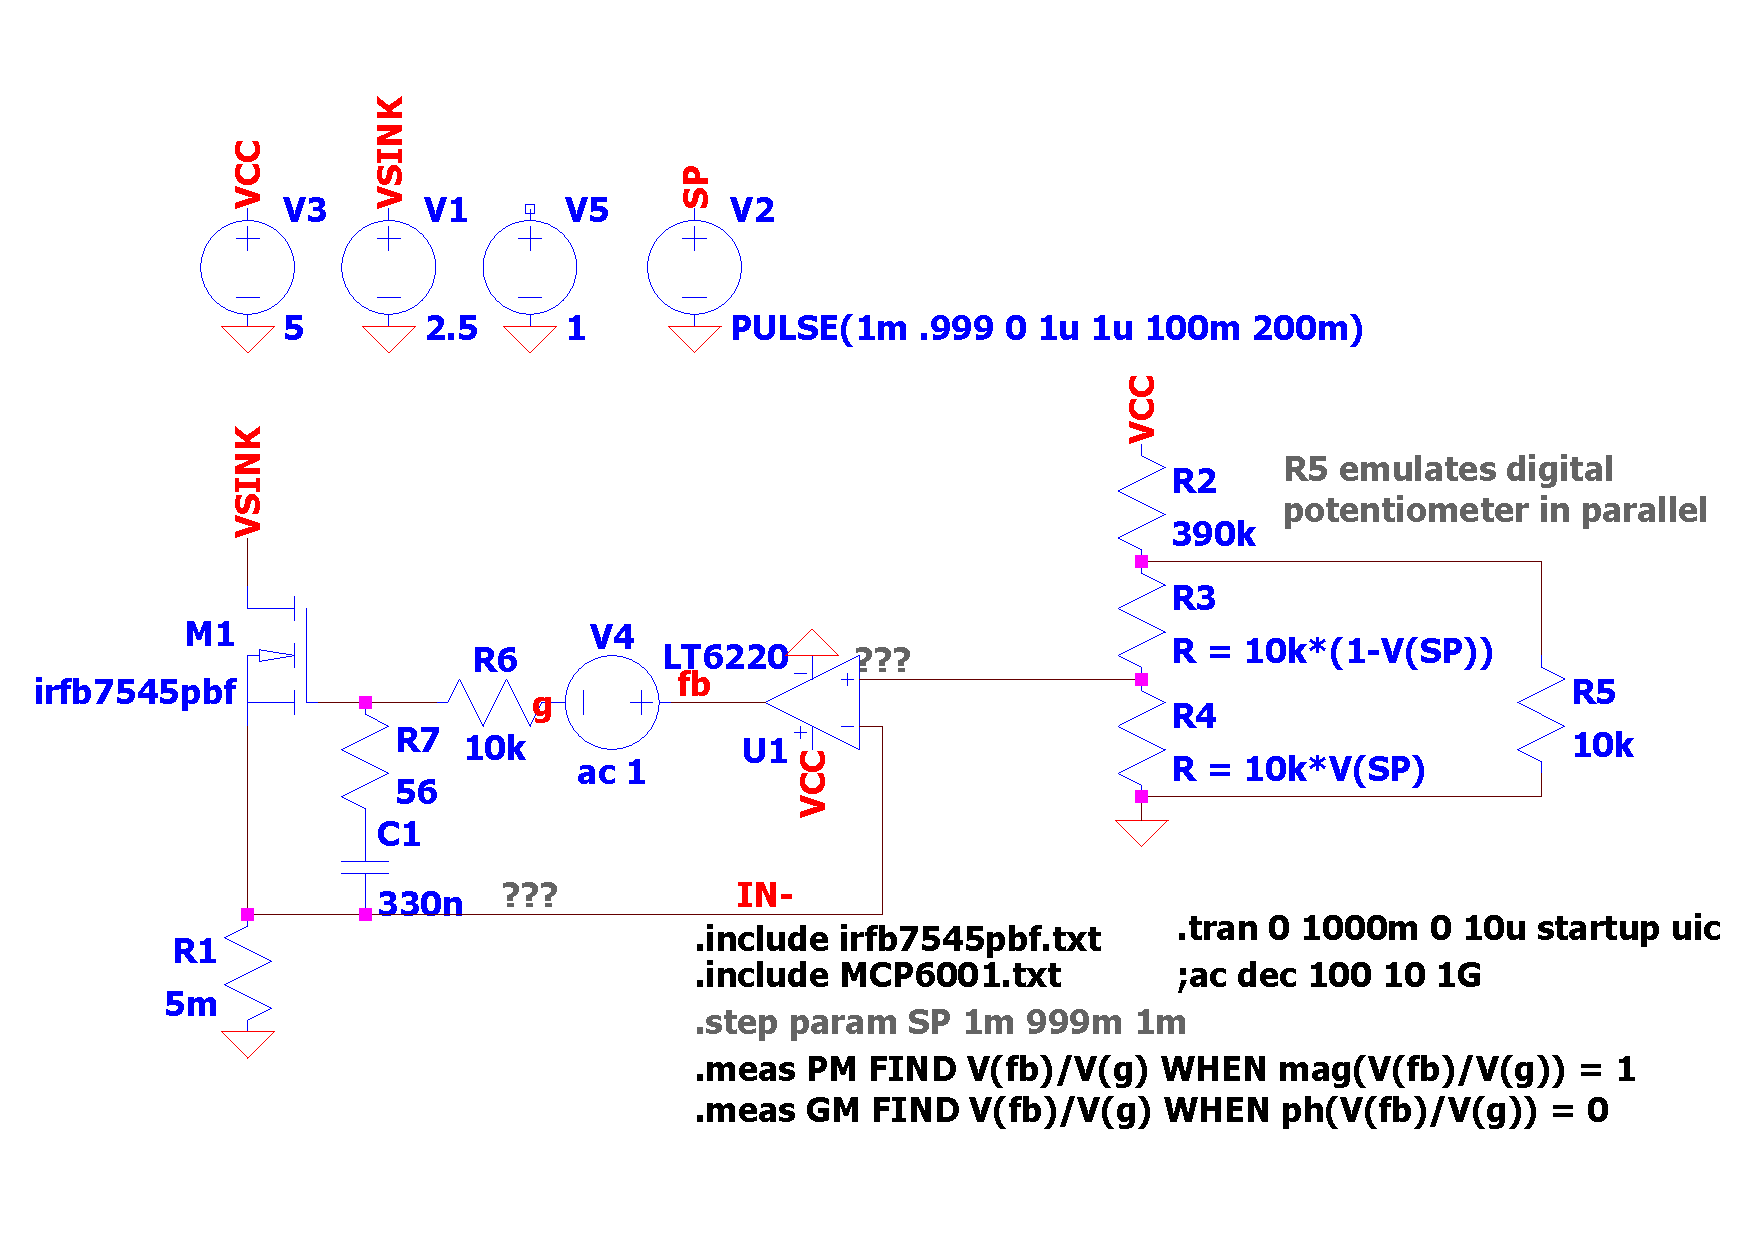
\includegraphics[width=0.45\textwidth]{CurrentSinkSchematic.pdf}
    \caption{12 A current sink schematic.}
    \label{fig:CurrentSinkSchematic}
\end{figure}

The corresponding KiCAD schematic is shown in Fig. \ref{fig:CellBoardKiCADSchematic}.

A model board has been made that interconnects all cell boards and incorporates a Atmega328PB MCU to control everything. The full schematic of this board is shown in Fig. \ref{fig:ModelBoardKiCADSchematic}. 

The mandatory reverse polarity protection on the model board is accomplished by adding a diode in series with the incoming supply rail.

\subsubsection{PCB design}
Since there are some substantial currents flowing through the design of up to 12 A, the trace widths have been determined according to IPC2221A at a maximum temperature rise of 10 \textdegree C.

Since all cell boards must be able to be placed in series, they should all be floating and be able to withstand at least the maximum expected cell voltage of each cell multiplied by the total amount of cells. Therefore, the minimum width of the isolation barrier has also been determined using IPC2221A.

